\documentclass[10pt]{article}
\usepackage[margin=0.72in]{geometry}
\usepackage[T1]{fontenc}
\usepackage{lmodern,microtype,booktabs,graphicx,xcolor,hyperref,placeins}
\definecolor{navy}{HTML}{16324F}\definecolor{teal}{HTML}{087E8B}\definecolor{violet}{HTML}{7C3AED}
\hypersetup{colorlinks=true,linkcolor=navy,urlcolor=teal}
\title{\textcolor{navy}{When Supervised Drift Detectors Need Exploration}\\[3pt]
\large An Early--Midpoint Audit Sensitivity for Delayed ADWIN}
\author{23I-2581 and 23I-2604\\Data Analysis and Visualization --- Phase 3 research addendum}
\date{18 November 2026}
\begin{document}\maketitle
\begin{abstract}
We investigate whether placing two label-independent audit probes at stream batches 1 and 12 enables canonical River ADWIN to operate under strict audit caps. The exploratory replay uses the same frozen prediction streams, truth, 30 seeds, seven conditions, four feedback delays, three cohort budgets and exact-quota/strict-cap rules as the one-probe baseline. With the corrected schedule, ADWIN fires in 273/630 strict-cap cells at delays 0 and 5, compared with zero under one probe. This comes with greater audit use (2.29--2.38 versus one cohort on average); it is not an equal-spend detector comparison. At delays 20 and 100, the 24-batch horizon still prevents timely error feedback.\end{abstract}
\section{Question and protocol}
The previous strict-cap result exposed a cold-start deadlock: one bootstrap cohort was insufficient for an error-change detector to request a second cohort. We therefore tested a fixed, label-independent pair at batches 1 and 12. Each selected cohort has 500 rows, and the detector receives row-level zero/one prediction errors only after that cohort's labels are released. Source batch $s$ is usable at decision clock $t$ iff $s+d<t$. The cohort budget is 2, 4 or 8; probes are selected only while a cohort remains available. All other settings match the River 0.27.0 ADWIN baseline ($\delta=0.002$, \texttt{clock=1}).

This was a post-hoc exploratory sensitivity motivated by the prior one-probe and adjacent-probe findings. It reuses the same cached streams and is not independent confirmation. The one-probe contrast is paired by seed after averaging seven conditions and three budgets; a 2,000-replicate seed bootstrap forms the intervals. Under strict caps, the probe pair changes audit volume, so episode-yield changes combine feedback opportunity and spend.
\section{Results}
\begin{figure}[ht]
\centering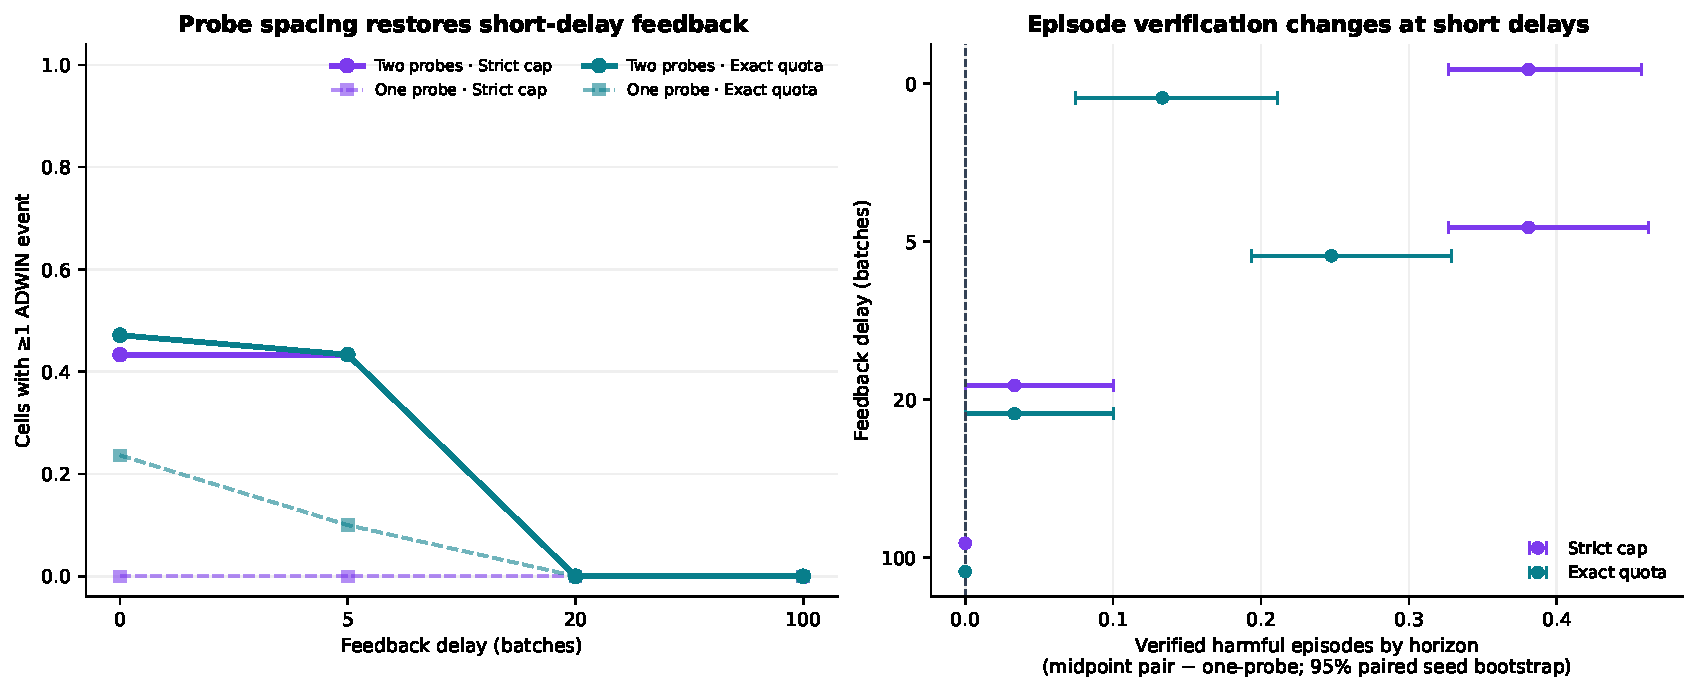
\includegraphics[width=\linewidth]{midpoint_probe_effects.pdf}
\caption{Left: fraction of seed--condition--budget cells with an ADWIN event, comparing the one-probe and corrected early--midpoint schedules. Right: paired change in harmful episodes verified by stream end; intervals resample 30 seeds after averaging matched conditions and budgets. Detection is not equivalent to correct harm localization.}
\end{figure}
\begin{table}[ht]
\centering\small\begin{tabular}{@{}llrrrr@{}}\toprule
Cost mode & Delay & One-probe events & Two-probe events & Mean audits & Verified episodes\\\midrule
exact quota & 0 & 149/630 & 297/630 & 4.67 & 0.646 \\
exact quota & 5 & 63/630 & 273/630 & 4.67 & 0.571 \\
exact quota & 20 & 0/630 & 0/630 & 4.67 & 0.033 \\
exact quota & 100 & 0/630 & 0/630 & 4.67 & 0.000 \\
strict cap & 0 & 0/630 & 273/630 & 2.29 & 0.571 \\
strict cap & 5 & 0/630 & 273/630 & 2.38 & 0.571 \\
strict cap & 20 & 0/630 & 0/630 & 2.00 & 0.033 \\
strict cap & 100 & 0/630 & 0/630 & 2.00 & 0.000 \\\bottomrule\end{tabular}
\caption{Counts are out of 630 seed--condition--budget cells per delay and cost mode. Mean audits and verified episodes are descriptive means across those cells.}\end{table}
\FloatBarrier
\section{Interpretation}
The corrected pair prevents the strict-cap deadlock for short feedback delays: the detector obtains a second error sample at batch 12, and events occur in 273/630 cells at delay 0 and 273/630 at delay 5. The corresponding paired change in verified episodes versus one probe is +0.381 (95\% seed-bootstrap interval 0.327--0.457) at both delays. However, mean strict-cap audit use rises from 1.00 to 2.29 and 2.38 cohorts, respectively. These differences therefore do not isolate detector quality at equal cost. Under exact quotas, audit volume is fixed; paired episode changes are +0.133 (0.075--0.211) at delay 0 and +0.248 (0.194--0.329) at delay 5. For delays 20 and 100, no ADWIN events occur: released supervision is too late relative to the 24-batch observation horizon.

The v1 exploratory output is retained but superseded. Its implementation incorrectly compared a batch clock with a cohort count, causing the batch-12 probe to be skipped for all declared budgets. The v2 runner gates probes on remaining cohort capacity, and its contract tests verify both probes are selected, budget caps hold, delayed labels are not ingested early, and output hashes match.
\section{Limits and implications}
This result supports only a narrow engineering conclusion: supervised drift monitoring under sparse delayed labels needs an explicit exploration or bootstrap policy. It does not show that ADWIN is generally effective, that fixed probes are optimal, or that they outperform alternative detectors. The schedule consumes budget before evidence of harm and can waste audits in stationary streams; this report does not estimate acquisition cost or deployment utility. All comparisons reuse synthetic cached streams; no natural-stream transfer, causal attribution, analyst benefit or human-subject claim is made. A prospectively locked exploration policy and equal-spend comparison are appropriate next experiments.
\section{Reproduction}
From the project root:
\begin{verbatim}
python scripts/run_adwin_midpoint_probe_sensitivity.py
python scripts/report_adwin_midpoint_probe_sensitivity.py
python -m pytest tests/phase3/test_adwin_audit_baseline_contract.py -q
\end{verbatim}
The run lock records code/data/output SHA-256 hashes, dependencies, probe clocks, seeds and runtime. The TeX source compiles with Tectonic and the receipt records the generated figure and PDF hashes.
\end{document}
